\documentclass[11pt]{article}
\usepackage{mathunal-base}
\mathunalfuente{serif}

\begin{document}

{\large\bfseries Parcial Final de Matemáticas Básicas --- Semestre 01-2019}

\medskip
\noindent Escuela de Matemáticas. Universidad Nacional de Colombia, Sede Medellín.

\medskip
\noindent\textit{Examen de selección múltiple con única respuesta. Marque una sola opción por pregunta.}

\begin{enumerate}
\item Sea $f$ la función definida por $f(x) = \begin{cases} x + 1 & \text{si } x \leq 2 \\ x^2 - 1 & \text{si } x > 3 \end{cases}$. Entonces, para $x > 3$, $\dfrac{f(x) - f(2)}{x - 2}$ es igual a:
\begin{opciones}
\item $1$
\item $x + 2$
\item $\dfrac{x^2 - 2}{x - 2}$
\item $\dfrac{x - 9}{x - 2}$
\end{opciones}

\item Cuatro hamburguesas y dos malteadas cuestan \$90. Las dos malteadas cuestan \$2,5 más que una hamburguesa. Si $x$ es el precio de una hamburguesa y $y$ es el costo de una malteada, las ecuaciones con las que se puede encontrar el costo de cada hamburguesa y cada malteada son:
\begin{opciones}
\item $4x + 2y = 90$, \quad $x + 2y = 2{,}5$
\item $4x + 2y = 90$, \quad $2y - x = 2{,}5$
\item $2x + 4y = 90$, \quad $2y - x = 2{,}5$
\item $2x + 4y = 90$, \quad $x + 2y = 2{,}5$
\end{opciones}

\item Sea $P(x)$ un polinomio de grado 3 con ceros $1$, $-2$ y $3$, tal que $P(4) = 2$. Entonces el polinomio $P(x)$ es:
\begin{opciones}
\item $4(x - 1)(x + 2)(x - 3)$
\item $\tfrac{1}{9}(x - 1)(x + 2)(x - 3)$
\item $\tfrac{1}{35}(x + 1)(x - 2)(x - 3)$
\item $\tfrac{1}{35}(x + 1)(x - 2)(x + 3)$
\end{opciones}

\item El dominio de la función definida por $f(x) = \ln\!\left(1 - \sqrt{1 - x}\right)$ es:
\begin{opciones}
\item $(-\infty, 1]$
\item $(-\infty, 0)$
\item $(0, 1]$
\item $(1, \infty)$
\end{opciones}

\item Si $\operatorname{sen} x = m$ y $\cos x < 0$ entonces $\operatorname{sen}(2x)$ es:
\begin{opciones}
\item $-2m\sqrt{1 - m^2}$
\item $2m\sqrt{1 - m^2}$
\item $-2\sqrt{1 - m^2}$
\item $2m$
\end{opciones}

\item El valor de $\cos 48^\circ \cos 18^\circ + \operatorname{sen} 48^\circ \operatorname{sen} 18^\circ$ es:
\begin{opciones}
\item $\tfrac{1}{2}$
\item $\tfrac{\sqrt3}{2}$
\item $-\tfrac{1}{2}$
\item $\cos(66^\circ)$
\end{opciones}

\item La ecuación de la recta que pasa por el punto $\left(-\tfrac{2}{3}, \tfrac{3}{2}\right)$ y es paralela a la recta de ecuación $3x - 2y + 6 = 0$ es:
\begin{opciones}
\item $y = -2x + \tfrac{1}{6}$
\item $y = -\tfrac{3}{2}x + \tfrac{1}{2}$
\item $y = -3x - \tfrac{1}{2}$
\item $y = \tfrac{3}{2}x + \tfrac{5}{2}$
\end{opciones}

\item El dominio de la función $f(x) = \sqrt{x + 1} + \dfrac{1}{x}$ es:
\begin{opciones}
\item $\mathbb{R} - \{0\}$
\item $\{x \in \mathbb{R} : x \geq -1,\ x \neq 0\}$
\item $\{x \in \mathbb{R} : x > 0\}$
\item $\{x \in \mathbb{R} : x \geq -1\}$
\end{opciones}

\item Si $\tan\theta = -\tfrac{3}{4}$ y $\operatorname{sen}\theta > 0$ entonces $\cos\theta$ es:
\begin{opciones}
\item $\tfrac{4}{5}$
\item $-\tfrac{4}{5}$
\item $\tfrac{5}{4}$
\item $-\tfrac{5}{4}$
\end{opciones}

\item El valor del discriminante de la ecuación $3z^2 + 12z = -7$ es:
\begin{opciones}
\item $30$
\item $60$
\item $50$
\item $20$
\end{opciones}

\item Al ordenar los números $\tfrac{80}{39}$, $\tfrac{83}{30}$ y $\tfrac{27}{13}$ afirmamos que:
\begin{opciones}
\item $\tfrac{80}{39} < \tfrac{27}{13} < \tfrac{83}{39}$
\item $\tfrac{27}{13} < \tfrac{80}{39} < \tfrac{83}{39}$
\item $\tfrac{80}{39} < \tfrac{83}{39} < \tfrac{27}{13}$
\item $0 < \tfrac{83}{39} < \tfrac{81}{39}$
\end{opciones}

\item El operario de un faro observa un barco en el mar con un ángulo de depresión de $30^\circ$, como se muestra en la siguiente figura. Si el barco se encuentra a $300$ m de la base del faro, entonces la altura del faro es:
\begin{center}
\begin{tikzpicture}[scale=1]
  \coordinate (B) at (0,0);
  \coordinate (P) at (7,0);
  \coordinate (T) at (7,2.4);
  \draw (B) -- (P) -- (T) -- cycle;
  \draw[very thick] (P) -- (T) node[midway,right=2pt] {$h$};
  \draw (B) -- (P) node[midway,below] {$300$ m};
  \draw ($(T)+(-1.2,0)$) -- (T);
  \draw ($(T)+(-0.7,0)$) arc (180:180+16:0.7);
  \node at ($(T)+(-1.0,-0.22)$) {\scriptsize $30^\circ$};
\end{tikzpicture}
\end{center}
\begin{opciones}
\item $100\sqrt3$
\item $150\sqrt3$
\item $300\sqrt3$
\item $600\sqrt3$
\end{opciones}

\item La inversa de la función $f(x) = \dfrac{2x - 1}{3 - x} + 1$ con dominio $D_f = \mathbb{R} - \{3\}$ es:
\begin{opciones}
\item $f^{-1}(x) = 3 - \dfrac{5}{x + 1}$ \; con $x \in \mathbb{R} - \{-1\}$
\item $f^{-1}(x) = \dfrac{3x - 3}{x + 1}$ \; con $x \in \mathbb{R} - \{-1\}$
\item $f^{-1}(x) = 3 + \dfrac{5}{x + 1}$ \; con $x \in \mathbb{R} - \{-1\}$
\item $f^{-1}(x) = \dfrac{3x + 1}{x + 2}$ \; con $x \in \mathbb{R} - \{-2\}$
\end{opciones}

\item La expresión $3\log_2 x - 7\log_2 x^3 + \log_2 z$ es igual a:
\begin{opciones}
\item $\log_2\!\left(3x - 7x^3 + z\right)$
\item $\log_2\!\left(21x^4 z\right)$
\item $\log_2\!\left(x - x^{21}\right)z$
\item $\log_2\!\left(\dfrac{z}{x^{18}}\right)$
\end{opciones}

\item Si $f(x) = \dfrac{x + 2}{x - 2}$, el valor de $f(f(a))$ (con $a \neq 2$ y $a \neq 6$) es:
\begin{opciones}
\item $\dfrac{a + 2}{a - 2}$
\item $-\dfrac{3a - 2}{a - 6}$
\item $\dfrac{a + 2}{a - 2} + 2$
\item $\dfrac{3a - 2}{a - 6}$
\end{opciones}

\item En la figura, $BD$ es una altura del triángulo $\triangle ABC$, y $EC$ es paralelo a $BD$. Además $\angle BCE = 8^\circ$, $\angle BAC = 30^\circ$, y $|AC| = 100$. Si $x = |BC|$ y $y = |AB|$ entonces la relación correcta es:
\begin{center}
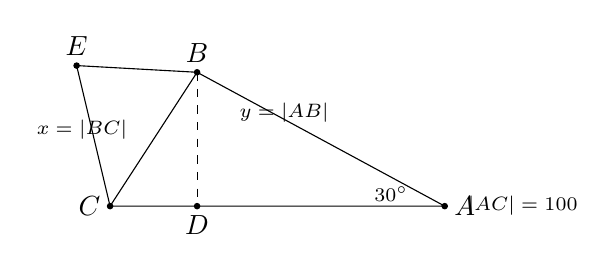
\begin{tikzpicture}[scale=0.85]
  \coordinate (A) at (5,0);
  \coordinate (C) at (0,0);
  \coordinate (D) at (1.3,0);
  \coordinate (B) at (1.3,2);
  \coordinate (E) at (-0.5,2.1);
  \draw (A) -- (B) -- (C) -- cycle;
  \draw[dashed] (B) -- (D);
  \draw (E) -- (C);
  \draw (E) -- (B);
  \foreach \p/\pos in {A/right,B/above,C/left,D/below,E/above} \fill (\p) circle (1.4pt) node[\pos] {$\p$};
  \node at (4.2,0.18) {\scriptsize $30^\circ$};
  \node[right] at (5.2,0) {\scriptsize $|AC| = 100$};
  \node at (2.6,1.4) {\scriptsize $y = |AB|$};
  \node[left] at (0.4,1.15) {\scriptsize $x = |BC|$};
\end{tikzpicture}
\end{center}
\begin{opciones}
\item $\operatorname{sen} 30^\circ = \dfrac{x}{y}$
\item $\dfrac{\operatorname{sen} 30^\circ}{y} = \dfrac{\operatorname{sen} 82^\circ}{100}$
\item $\dfrac{\operatorname{sen} 30^\circ}{x} = \dfrac{\operatorname{sen} 82^\circ}{y}$
\item $\dfrac{\operatorname{sen} 30^\circ}{y} = \dfrac{\operatorname{sen} 68^\circ}{100}$
\end{opciones}
\end{enumerate}

\vfill
\noindent{\small\itshape Transcripción digital --- MathUNAL}

\end{document}
